\documentclass[10pt]{beamer}
\usetheme{metropolis}

% ── Packages ──
\usepackage{amsmath,amssymb,amsthm}
\usepackage{tikz}
\usetikzlibrary{positioning,arrows.meta,fit,matrix,backgrounds,calc}
\usepackage{graphicx}
\usepackage{array}
\usepackage{etoolbox}

% ── Theorem environments ──
\theoremstyle{definition}
\newtheorem{defi}{Definition}[section]
\newtheorem{prop}{Proposition}[section]
\newtheorem{thm}{Theorem}[section]
\newtheorem{cor}{Corollary}[section]

% Custom theorem styles with colors
\setbeamercolor{block title}{bg=red!75!black,fg=white}
\setbeamercolor{block body}{bg=yellow!10!white}

% Proposition uses yellow title
\AtBeginEnvironment{prop}{%
  \setbeamercolor{block title}{bg=yellow!75!black,fg=black}%
  \setbeamercolor{block body}{bg=yellow!10!white}%
}
\AtEndEnvironment{prop}{%
  \setbeamercolor{block title}{bg=red!75!black,fg=white}%
}

% Theorem uses yellow title
\AtBeginEnvironment{thm}{%
  \setbeamercolor{block title}{bg=yellow!75!black,fg=black}%
  \setbeamercolor{block body}{bg=yellow!10!white}%
}
\AtEndEnvironment{thm}{%
  \setbeamercolor{block title}{bg=red!75!black,fg=white}%
}

% ── Emoji definitions ──
\newcommand{\bean}{
\includegraphics[scale=0.07]{Pictures/bean.png}}
\newcommand{\leaf}{
\includegraphics[scale=0.08]{Pictures/leaf.png}}
\newcommand{\lemon}{
\includegraphics[scale=0.08]{Pictures/lemon.png}}
\newcommand{\cow}{
\includegraphics[scale=0.08]{Pictures/cow.png}}
\newcommand{\milk}{
\includegraphics[scale=0.08]{Pictures/milk.png}}
\newcommand{\coffee}{
\includegraphics[scale=0.08]{Pictures/coffee.png}}
\newcommand{\tea}{
\includegraphics[scale=0.08]{Pictures/tea.png}}
\newcommand{\bento}{
\includegraphics[scale=0.08]{Pictures/bento.png}}
\newcommand{\ramen}{\includegraphics[scale=0.08]{Pictures/ramen.png}}
\newcommand{\cola}{
\includegraphics[scale=0.08]{Pictures/cola.png}}

% ── Highlighting ──
\newcommand{\x}[1]{\alert{\textbf{#1}}}

\title{Lecture 5: Solving Linear Equations and Null Space}
\subtitle{MATH203 Applied Linear Algebra}
\date{}

\begin{document}
\maketitle

% ═══════════════════════════════════════
% §0 MOTIVATION
% ═══════════════════════════════════════
\section{Motivation: Why We Need to Solve Equations}

\begin{frame}{Recall: The Two Languages (Lecture 4)}

Every subspace has \x{two complementary descriptions}:

\vspace{1em}

\begin{center}
\begin{tabular}{|c|c|c|}
\hline
\textbf{Language} & \textbf{How it works} & \textbf{Example} \\
\hline
\x{Descriptive} & List \textbf{equations} & $\{\mathbf{x} : A\mathbf{x} = \mathbf{0}\}$ \\
 & (constraints) & \\
\hline
\x{Constructive} & Provide \textbf{recipe} & $\text{span}\{\mathbf{v}_1, \mathbf{v}_2, \ldots\}$ \\
 & (generate members) & \\
\hline
\end{tabular}
\end{center}

\vspace{1em}

\x{Today's question}: What is each language \textbf{good at}? What is each language \textbf{bad at}?

\end{frame}

\begin{frame}{Each Language Has Strengths and Weaknesses}

\begin{center}
\begin{tabular}{|c|c|c|}
\hline
& \x{Descriptive} & \x{Constructive} \\
& $\{\mathbf{x} : A\mathbf{x} = \mathbf{0}\}$ & $\text{span}\{\mathbf{v}_1, \ldots\}$ \\
\hline
\textbf{Good at} & Verification & Generation \\
 & (check membership) & (produce members) \\
\hline
\textbf{Bad at} & Generation & Verification \\
 & (find examples) & (check membership) \\
\hline
\end{tabular}
\end{center}

\vspace{1em}

\x{Key insight}: \textbf{Solving equations helps both languages do what they're bad at!}

\vspace{1em}

Let's see two concrete examples using Shinchan's coffee shop$\ldots$

\end{frame}

\begin{frame}{Example Setup: Shinchan's Coffee Shop Menu}

Shinchan has three drinks on his menu:

\vspace{0.5em}

\begin{center}
\begin{tabular}{c|ccc}
& \milk{} milk & \coffee{} coffee & \tea{} tea \\
\hline
\leaf{} tea leaves & 0 & 0 & 2 \\
\lemon{} lemon & 0 & 0 & 1 \\
\bean{} beans & 0 & 2 & 4 \\
\cow{} milk & 1 & 0 & 1 \\
\end{tabular}
\end{center}

\vspace{0.5em}

Matrix form:
$$A = \begin{pmatrix}
0 & 0 & 2 \\
0 & 0 & 1 \\
0 & 2 & 4 \\
1 & 0 & 1
\end{pmatrix}$$

\end{frame}

\begin{frame}{Case 1: Column Space (Naturally Constructive)}

The column space is \x{naturally constructive}:

$$\text{Col}(A) = \text{span}\left\{\begin{pmatrix} 0\\0\\0\\1 \end{pmatrix}, \begin{pmatrix} 0\\0\\2\\0 \end{pmatrix}, \begin{pmatrix} 2\\1\\4\\1 \end{pmatrix}\right\}$$

These are the ingredient lists for \milk, \coffee, \tea.

\vspace{1em}

\x{In coffee shop language}: $\text{Col}(A)$ = \textbf{all possible ingredient combinations we can produce from our menu}.

\end{frame}

\begin{frame}{Case 1: Generation is Easy}

\x{Generation} (easy): Want a vector in $\text{Col}(A)$?

\vspace{0.5em}

Just pick a combination of drinks!

$$2\text{\milk} + 3\text{\coffee} = 2\begin{pmatrix} 0\\0\\0\\1 \end{pmatrix} + 3\begin{pmatrix} 0\\0\\2\\0 \end{pmatrix} = \begin{pmatrix} 0\\0\\6\\2 \end{pmatrix}$$

\vspace{0.5em}

\x{In coffee shop language}: "Make 2 glasses of milk and 3 cups of coffee" produces an ingredient combination in $\text{Col}(A)$.

\vspace{1em}

Generation = \x{making products}. Easy with constructive description!

\end{frame}

\begin{frame}{Case 1: Verification is Hard}

\x{Verification} (hard): A customer brings an ingredient list $\mathbf{b} = \begin{pmatrix} 4\\2\\10\\3 \end{pmatrix}$.

\vspace{0.5em}

\x{Question in coffee shop language}: \textbf{Can we make a drink combination that uses exactly these ingredients?}

\vspace{0.5em}

This is asking: Is $\mathbf{b} \in \text{Col}(A)$?

\vspace{1em}

Can't tell by looking! Need to \x{solve}: $A\mathbf{x} = \mathbf{b}$

\begin{itemize}
\item If solution exists $\Rightarrow$ Yes, we can make it! ($\mathbf{b} \in \text{Col}(A)$)
\item If no solution $\Rightarrow$ No, impossible with our menu ($\mathbf{b} \notin \text{Col}(A)$)
\end{itemize}

\vspace{0.5em}

\x{Solving equations gives constructive description the power to verify!}

\end{frame}

\begin{frame}{Case 2: Null Space (Naturally Descriptive)}

The null space is \x{naturally descriptive}:

$$\text{Null}(A) = \{\mathbf{x} \in \mathbb{R}^3 : A\mathbf{x} = \mathbf{0}\}$$

\vspace{1em}

\x{In coffee shop language}: $\text{Null}(A)$ = \textbf{records of relationships between drinks}.

\vspace{0.5em}

For example: If \tea{} can be made from 2×\coffee, then the relationship is recorded as:

$$\begin{pmatrix} 0 \\ 2 \\ -1 \end{pmatrix}: \quad \text{2 coffees can make 1 tea}$$

\vspace{0.5em}

\x{Geometric meaning}: $\text{Null}(A)$ stores all \textbf{relationships between the columns}.

\end{frame}

\begin{frame}{Case 2: Verification is Easy (Coffee Shop Example)}

\x{Verification} (easy): Someone claims "\tea{} can be made from 1 \milk{} and 1 \coffee."

\vspace{0.5em}

Is this relationship valid? Check if $\mathbf{v} = \begin{pmatrix} 1\\1\\-1 \end{pmatrix} \in \text{Null}(A)$:

\vspace{0.5em}

Compute:
\begin{align*}
1\text{\milk} + 1\text{\coffee} - 1\text{\tea} &= \begin{pmatrix} 0\\0\\0\\1 \end{pmatrix} + \begin{pmatrix} 0\\0\\2\\0 \end{pmatrix} - \begin{pmatrix} 2\\1\\4\\1 \end{pmatrix} \\
&= \begin{pmatrix} -2\\-1\\-2\\0 \end{pmatrix} \neq \mathbf{0}
\end{align*}

\x{Coffee shop conclusion}: This is NOT a valid relationship! \tea{} cannot be made from 1 \milk{} and 1 \coffee.

\end{frame}

\begin{frame}{Case 2: Generation is Hard}

\x{Generation} (hard): Looking at the menu, can you find the relationships?

\begin{center}
\begin{tabular}{c|ccc}
& \milk & \coffee & \tea \\
\hline
\leaf & 0 & 0 & 2 \\
\lemon & 0 & 0 & 1 \\
\bean & 0 & 2 & 4 \\
\cow & 1 & 0 & 1 \\
\end{tabular}
\end{center}

\x{Question in coffee shop language}: \textbf{Which drinks can be made from others? What are the relationships?}

\vspace{0.5em}

Hard to see by staring! Need to \x{solve} $A\mathbf{x} = \mathbf{0}$.

\end{frame}

\begin{frame}{Case 2: Solving Reveals the Relationship}

After solving $A\mathbf{x} = \mathbf{0}$ (we'll learn how soon):

$$\text{Null}(A) = \text{span}\left\{\begin{pmatrix} 0\\2\\-1 \end{pmatrix}\right\}$$

\vspace{0.5em}

\x{What does this tell us in coffee shop language?}

$$\begin{pmatrix} 0 \\ 2 \\ -1 \end{pmatrix}: \quad \text{\tea{} can be made from 2 \coffee}$$

\vspace{1em}

\x{Aha!} This is the \textbf{relationship}: 1 cup of \tea{} uses exactly the same ingredients as 2 cups of \coffee.

\vspace{1em}

\x{Solving equations gives descriptive description the power to generate relationships!}

\end{frame}

\begin{frame}{Summary: The Power of Solving Equations}

\begin{center}
\begin{tabular}{|c|c|c|}
\hline
\textbf{Subspace} & \textbf{Weakness} & \textbf{Solving provides} \\
\hline
$\text{Col}(A)$ & Verification & Solve $A\mathbf{x}=\mathbf{b}$ \\
(constructive) & "Can we make this?" & to check if possible \\
\hline
$\text{Null}(A)$ & Generation & Solve $A\mathbf{x}=\mathbf{0}$ \\
(descriptive) & "What relationships?" & to find relationships \\
\hline
\end{tabular}
\end{center}

\vspace{1em}

\x{Today's focus}: Develop a \textbf{cross-filling method} to solve $A\mathbf{x} = \mathbf{b}$, which:

\begin{itemize}
\item Finds all relationships between products (basis for $\text{Null}(A)$)
\item Checks if a product is possible ($\mathbf{b} \in \text{Col}(A)$?)
\item Determines uniqueness (Is there only one way?)
\end{itemize}

\end{frame}

% ═══════════════════════════════════════
% §1 NULL SPACE
% ═══════════════════════════════════════
\section{Null Space: The Relationship Catalog}

\begin{frame}{Definition: Null Space}

\begin{defi}[Null Space (Kernel)]
For a matrix $A \in \mathbb{R}^{m \times n}$, the \x{null space} is:

$$\text{Null}(A) = \{\mathbf{x} \in \mathbb{R}^n : A\mathbf{x} = \mathbf{0}\}$$

\textbf{Meaning}: $\text{Null}(A)$ records all \x{relationships between the columns} of $A$.

Also called the \x{kernel}, denoted $\ker(A)$.
\end{defi}

\vspace{0.5em}

\x{In coffee shop language}: Drink combinations that reveal "which drinks can be made from others."

\end{frame}

\begin{frame}{Immediate Example: Is This a Valid Relationship?}

From Shinchan's menu ($A$ from before), someone claims:

"\tea{} can be made from 2 \coffee"

\vspace{0.5em}

This means: $\begin{pmatrix} 0 \\ 2 \\ -1 \end{pmatrix}$ should be in $\text{Null}(A)$.

\vspace{0.5em}

Let's verify:

$$A\begin{pmatrix} 0 \\ 2 \\ -1 \end{pmatrix} = 0 \cdot \begin{pmatrix} 0\\0\\0\\1 \end{pmatrix} + 2 \cdot \begin{pmatrix} 0\\0\\2\\0 \end{pmatrix} - 1 \cdot \begin{pmatrix} 2\\1\\4\\1 \end{pmatrix} = \begin{pmatrix} -2\\-1\\0\\-1 \end{pmatrix} \neq \mathbf{0}$$

\x{Result}: This is NOT a valid relationship! (Actually \tea{} $\neq$ 2×\coffee)

\end{frame}

\begin{frame}{What Would Be a Valid Relationship?}

Let's try another: someone claims "\tea{} can be made from 2 \coffee{} plus 1 \milk"

\vspace{0.5em}

This means: $\begin{pmatrix} 1 \\ 2 \\ -1 \end{pmatrix}$ might be in $\text{Null}(A)$.

$$A\begin{pmatrix} 1 \\ 2 \\ -1 \end{pmatrix} = \begin{pmatrix} 0\\0\\0\\1 \end{pmatrix} + 2\begin{pmatrix} 0\\0\\2\\0 \end{pmatrix} - \begin{pmatrix} 2\\1\\4\\1 \end{pmatrix} = \begin{pmatrix} -2\\-1\\0\\0 \end{pmatrix} \neq \mathbf{0}$$

\x{Still not valid!}

\vspace{0.5em}

How do we \x{systematically find} valid relationships? We need to solve $A\mathbf{x} = \mathbf{0}$!

\end{frame}

\begin{frame}{Key Insight: Null Space Records Relationships}

\x{Important}:

\begin{itemize}
\item Each vector $\mathbf{x} \in \text{Null}(A)$ records a relationship
\item $\text{Null}(A)$ = \textbf{"relationship catalog"} between columns
\end{itemize}

\vspace{1em}

\x{Size of the catalog}:
\begin{itemize}
\item $\text{Null}(A) = \{\mathbf{0}\}$ $\to$ no relationships $\to$ columns \textbf{independent}
\item $\dim(\text{Null}(A)) = k$ $\to$ there are $k$ independent relationships
\end{itemize}

\end{frame}

\begin{frame}{Null Space is a Subspace}

\begin{prop}
$\text{Null}(A)$ is a subspace of $\mathbb{R}^n$.
\end{prop}

\vspace{0.5em}

\textbf{Proof}: Verify the three axioms:

\begin{enumerate}
\item $\mathbf{0} \in \text{Null}(A)$ since $A\mathbf{0} = \mathbf{0}$ \checkmark
\item If $A\mathbf{x}_1 = \mathbf{0}$ and $A\mathbf{x}_2 = \mathbf{0}$, then
$$A(\mathbf{x}_1 + \mathbf{x}_2) = \mathbf{0}$$ \checkmark
\item If $A\mathbf{x} = \mathbf{0}$, then $A(c\mathbf{x}) = \mathbf{0}$ \checkmark
\end{enumerate}

\end{frame}

\begin{frame}{The Problem: We Need Constructive Description}

\x{Descriptive}: $\text{Null}(A) = \{\mathbf{x} : A\mathbf{x} = \mathbf{0}\}$

\begin{itemize}
\item \textbf{Verification} (easy): Is $\mathbf{v}$ a valid relationship? Compute $A\mathbf{v}$
\item \textbf{Generation} (hard): Find all relationships? Can't guess!
\end{itemize}

\vspace{1em}

\x{Goal}: Convert to \textbf{constructive}:

$$\text{Null}(A) = \text{span}\{\mathbf{v}_1, \mathbf{v}_2, \ldots, \mathbf{v}_k\}$$

\vspace{0.5em}

\x{Method}: Solve $A\mathbf{x} = \mathbf{0}$ using cross-filling!

\vspace{0.5em}

But first — to solve $A\mathbf{x} = \mathbf{b}$ in general, we need augmented matrices$\ldots$

\end{frame}

% ═══════════════════════════════════════
% §1.5 AUGMENTED MATRIX CONNECTION
% ═══════════════════════════════════════
\section{From $A\mathbf{x} = \mathbf{b}$ to Augmented Matrix}

\begin{frame}{Motivation: Why Augmented Matrix?}

We want to solve: $A\mathbf{x} = \mathbf{b}$

\vspace{1em}

\x{Column view}:
$$A\mathbf{x} = \begin{pmatrix} | & | & & | \\ \mathbf{a}_1 & \mathbf{a}_2 & \cdots & \mathbf{a}_n \\ | & | & & | \end{pmatrix} \begin{pmatrix} x_1 \\ x_2 \\ \vdots \\ x_n \end{pmatrix} = x_1\mathbf{a}_1 + x_2\mathbf{a}_2 + \cdots + x_n\mathbf{a}_n = \mathbf{b}$$

\vspace{0.5em}

We're looking for \x{coefficients} $x_1, \ldots, x_n$ that combine columns to get $\mathbf{b}$.

\vspace{1em}

\x{Key idea}: Add $\mathbf{b}$ as an extra column$\ldots$

\end{frame}

\begin{frame}{The Augmented Matrix}

Form the \x{augmented matrix}:

$$(A \mid \mathbf{b}) = \begin{pmatrix} | & | & & | & | \\ \mathbf{a}_1 & \mathbf{a}_2 & \cdots & \mathbf{a}_n & \mathbf{b} \\ | & | & & | & | \end{pmatrix}$$

\vspace{1em}

This is an $m \times (n+1)$ matrix with $n+1$ columns.

\vspace{1em}

Now: What happens if we take a linear combination with coefficients $\begin{pmatrix} x_1 \\ \vdots \\ x_n \\ -1 \end{pmatrix}$?

\end{frame}

\begin{frame}{The Key Connection}

Take $(A \mid \mathbf{b})$ and multiply by $\begin{pmatrix} x_1 \\ \vdots \\ x_n \\ -1 \end{pmatrix}$:

\vspace{0.5em}

$$(A \mid \mathbf{b}) \begin{pmatrix} x_1 \\ \vdots \\ x_n \\ -1 \end{pmatrix} = x_1\mathbf{a}_1 + \cdots + x_n\mathbf{a}_n + (-1)\mathbf{b}$$

\vspace{0.5em}

This equals $\mathbf{0}$ if and only if:

$$x_1\mathbf{a}_1 + \cdots + x_n\mathbf{a}_n = \mathbf{b}$$

which is exactly $A\mathbf{x} = \mathbf{b}$!

\end{frame}

\begin{frame}{Why This Matters}

\x{Crucial observation}:

$$A\mathbf{x} = \mathbf{b} \quad\text{has solution}\quad \iff \quad \begin{pmatrix} \mathbf{x} \\ -1 \end{pmatrix} \text{ records a relationship in } (A \mid \mathbf{b})$$

\vspace{1em}

But we won't compute $\text{Null}(A \mid \mathbf{b})$ directly. Instead:

\vspace{0.5em}

We'll use \x{cross-filling} on $(A \mid \mathbf{b})$ to extract simplified equations, then solve backwards!

\end{frame}

% ═══════════════════════════════════════
% §2 CROSS-FILLING METHOD
% ═══════════════════════════════════════
\section{The Cross-Filling Method for Solving $A\mathbf{x} = \mathbf{b}$}

\begin{frame}{Recall: Cross-Filling Decomposition (Lecture 3)}

Any matrix can be decomposed via cross-filling:

$$A = R_1 + R_2 + \cdots + R_r$$

where each $R_i$ is a \x{rank-one matrix}.

\vspace{1em}

\x{Key property}: All rows of a rank-one matrix are scalar multiples of each other.

\vspace{1em}

Example:
$$R = \begin{pmatrix} 2 \\ 1 \\ 3 \end{pmatrix} \begin{pmatrix} 1 & 2 & 3 \end{pmatrix} = \begin{pmatrix}
2 & 4 & 6 \\
1 & 2 & 3 \\
3 & 6 & 9
\end{pmatrix}$$

\end{frame}

\begin{frame}{Apply Cross-Filling to Augmented Matrix}

For $(A \mid \mathbf{b})$, we cross-fill:

$$(A \mid \mathbf{b}) = (R_1 \mid \mathbf{b}_1) + (R_2 \mid \mathbf{b}_2) + \cdots + (R_r \mid \mathbf{b}_r)$$

\vspace{1em}

Each piece $(R_i \mid \mathbf{b}_i)$ is a \x{rank-one augmented matrix} (includes both $A$ and $\mathbf{b}$ parts).

\vspace{1em}

\x{Key observation}: Since $(R_i \mid \mathbf{b}_i)$ is rank-one, all its rows are proportional — they represent the \x{same equation}!

\vspace{1em}

One rank-one piece = one independent equation.

\end{frame}

\begin{frame}{Why Are These Equations Valid?}

\x{Question}: Why is solving these $r$ equations equivalent to the original $m$ equations?

\vspace{1em}

\x{Answer}: Cross-filling gives $(A \mid \mathbf{b}) = UV$ where:
\begin{itemize}
\item $U$ is $m \times r$ with \textbf{linearly independent columns}
\item $V$ is $r \times (n+1)$
\end{itemize}

\vspace{0.5em}

Since $U$'s columns are independent:

$$UV\mathbf{z} = \mathbf{0} \iff UV\mathbf{z} = U\mathbf{0} \iff V\mathbf{z} = \mathbf{0}$$

\vspace{0.5em}

(Left multiplication by independent columns can be cancelled.)

\end{frame}

\begin{frame}{What is $V$ Explicitly?}

$$V = \begin{pmatrix}
\text{— row from } (R_1 \mid \mathbf{b}_1) \text{ —} \\
\text{— row from } (R_2 \mid \mathbf{b}_2) \text{ —} \\
\vdots \\
\text{— row from } (R_r \mid \mathbf{b}_r) \text{ —}
\end{pmatrix}$$

\vspace{0.5em}

$V$ is an $r \times (n+1)$ \x{augmented matrix}, where:
\begin{itemize}
\item Each row is one simplified equation
\item The last column corresponds to the right-hand side
\end{itemize}

\vspace{0.5em}

\x{In practice}: We'll see $V$ explicitly in our example!

\end{frame}

\begin{frame}{Observation: Variables Decrease}

As cross-filling proceeds, each piece has fewer active variables:

\begin{itemize}
\item $(R_1 \mid \mathbf{b}_1)$: involves \x{all $n$ variables}
\item $(R_2 \mid \mathbf{b}_2)$: involves \x{fewer variables} (at least column $j_1$ eliminated)
\item $(R_3 \mid \mathbf{b}_3)$: involves \x{even fewer variables}
\item $\vdots$
\item $(R_r \mid \mathbf{b}_r)$: involves \x{fewest variables}
\end{itemize}

\vspace{1em}

\x{Key}: Each successive piece has \textbf{at least one fewer variable} (possibly more, depending on which columns are eliminated).

\vspace{0.5em}

\x{Strategy}: Start from the end (fewest variables) and work backwards!

\end{frame}

% ═══════════════════════════════════════
% §3 CONCRETE EXAMPLE (VISUAL)
% ═══════════════════════════════════════
\section{Concrete Example: Step-by-Step Visual Cross-Filling}

\begin{frame}{Example Setup}

Solve:
$$A\mathbf{x} = \mathbf{b}$$

where

$$A = \begin{pmatrix}
1 & 2 & 0 & 1 \\
2 & 4 & 1 & 2 \\
3 & 6 & 1 & 3
\end{pmatrix}, \quad \mathbf{b} = \begin{pmatrix} 5 \\ 11 \\ 16 \end{pmatrix}$$

\vspace{1em}

Form augmented matrix $(A \mid \mathbf{b})$ and cross-fill visually!

\end{frame}

\begin{frame}[fragile]{Step 1: Initial Augmented Matrix}

\begin{center}
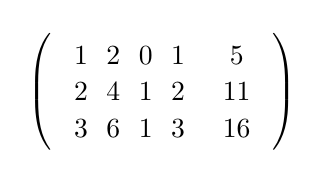
\begin{tikzpicture}[scale=0.7]
\matrix (m) [matrix of math nodes, left delimiter=(, right delimiter=), ampersand replacement=\&] {
1 \& 2 \& 0 \& 1 \& \vrule \& 5 \\
2 \& 4 \& 1 \& 2 \& \vrule \& 11 \\
3 \& 6 \& 1 \& 3 \& \vrule \& 16 \\
};
\end{tikzpicture}
\end{center}

\vspace{1em}

\x{Goal}: Use cross-filling to decompose into rank-one pieces.

\vspace{0.5em}

\x{Strategy}: Choose pivots to eliminate columns one by one.

\end{frame}

\begin{frame}[fragile]{Step 2: Choose First Pivot at (1,1)}

\begin{center}
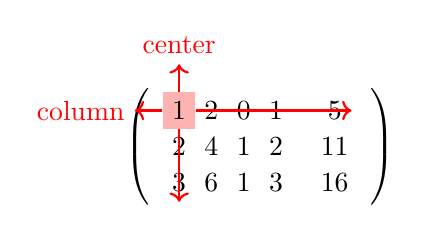
\begin{tikzpicture}[scale=0.7]
\matrix (m) [matrix of math nodes, left delimiter=(, right delimiter=), ampersand replacement=\&] {
|[fill=red!30]| 1 \& 2 \& 0 \& 1 \& \vrule \& 5 \\
2 \& 4 \& 1 \& 2 \& \vrule \& 11 \\
3 \& 6 \& 1 \& 3 \& \vrule \& 16 \\
};
% Draw cross
\draw[red, thick, ->] (m-1-1.north) -- ++(0, 0.5) node[above] {center};
\draw[red, thick, ->] (m-1-1.west) -- ++(-0.5, 0) node[left] {column};
\draw[red, thick, ->] (m-1-1.east) -- (m-1-6.east);
\draw[red, thick, ->] (m-1-1.south) -- (m-3-1.south);
\end{tikzpicture}
\end{center}

\vspace{0.5em}

Pivot = entry $(1,1) = 1$ (highlighted red).

\x{Extract}: Column $\begin{pmatrix} 1 \\ 2 \\ 3 \end{pmatrix}$ × Row $\begin{pmatrix} 1 & 2 & 0 & 1 & | & 5 \end{pmatrix}$

\end{frame}

\begin{frame}[fragile]{Step 3: First Rank-One Piece $(R_1 \mid \mathbf{b}_1)$}

$$(R_1 \mid \mathbf{b}_1) = \begin{pmatrix} 1 \\ 2 \\ 3 \end{pmatrix} \begin{pmatrix} 1 & 2 & 0 & 1 & | & 5 \end{pmatrix}$$

\vspace{0.5em}

Expanding:

\begin{center}
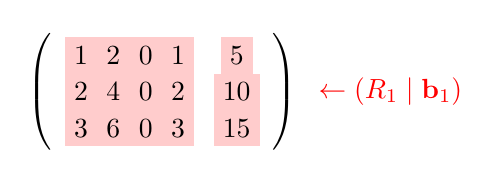
\begin{tikzpicture}[scale=0.7]
\matrix (m) [matrix of math nodes, left delimiter=(, right delimiter=), ampersand replacement=\&] {
|[fill=red!20]| 1 \& |[fill=red!20]| 2 \& |[fill=red!20]| 0 \& |[fill=red!20]| 1 \& \vrule \& |[fill=red!20]| 5 \\
|[fill=red!20]| 2 \& |[fill=red!20]| 4 \& |[fill=red!20]| 0 \& |[fill=red!20]| 2 \& \vrule \& |[fill=red!20]| 10 \\
|[fill=red!20]| 3 \& |[fill=red!20]| 6 \& |[fill=red!20]| 0 \& |[fill=red!20]| 3 \& \vrule \& |[fill=red!20]| 15 \\
};
\node[right=0.5cm of m, red] {$\leftarrow (R_1 \mid \mathbf{b}_1)$};
\end{tikzpicture}
\end{center}

\vspace{0.5em}

\x{Equation from $(R_1 \mid \mathbf{b}_1)$} (read any row, e.g., row 1):

$$x_1 + 2x_2 + 0x_3 + 1x_4 = 5$$

\end{frame}

\begin{frame}[fragile]{Step 4: Compute Remainder}

\x{Before}: $(A \mid \mathbf{b})$

\begin{center}
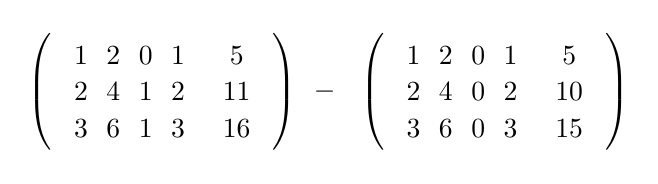
\begin{tikzpicture}[scale=0.7]
\matrix (m1) [matrix of math nodes, left delimiter=(, right delimiter=), ampersand replacement=\&] {
1 \& 2 \& 0 \& 1 \& \vrule \& 5 \\
2 \& 4 \& 1 \& 2 \& \vrule \& 11 \\
3 \& 6 \& 1 \& 3 \& \vrule \& 16 \\
};
\node at ($(m1.east) + (1,0)$) {$-$};
\matrix (m2) [right=1.5cm of m1, matrix of math nodes, left delimiter=(, right delimiter=), ampersand replacement=\&] {
1 \& 2 \& 0 \& 1 \& \vrule \& 5 \\
2 \& 4 \& 0 \& 2 \& \vrule \& 10 \\
3 \& 6 \& 0 \& 3 \& \vrule \& 15 \\
};
\end{tikzpicture}
\end{center}

\vspace{0.5em}

\x{After}: Remainder

\begin{center}
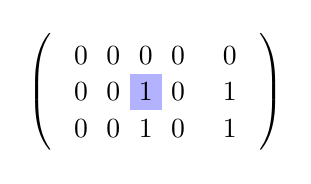
\begin{tikzpicture}[scale=0.7]
\matrix (m) [matrix of math nodes, left delimiter=(, right delimiter=), ampersand replacement=\&] {
0 \& 0 \& 0 \& 0 \& \vrule \& 0 \\
0 \& 0 \& |[fill=blue!30]| 1 \& 0 \& \vrule \& 1 \\
0 \& 0 \& 1 \& 0 \& \vrule \& 1 \\
};
\end{tikzpicture}
\end{center}

Column 1 eliminated! Next pivot at $(2,3)$ (blue).

\end{frame}

\begin{frame}[fragile]{Step 5: Choose Second Pivot at (2,3)}

\begin{center}
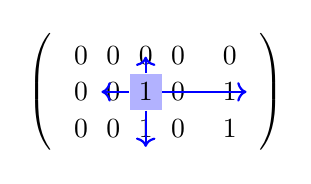
\begin{tikzpicture}[scale=0.7]
\matrix (m) [matrix of math nodes, left delimiter=(, right delimiter=), ampersand replacement=\&] {
0 \& 0 \& 0 \& 0 \& \vrule \& 0 \\
0 \& 0 \& |[fill=blue!30]| 1 \& 0 \& \vrule \& 1 \\
0 \& 0 \& 1 \& 0 \& \vrule \& 1 \\
};
% Draw cross
\draw[blue, thick, ->] (m-2-3.north) -- ++(0, 0.3);
\draw[blue, thick, ->] (m-2-3.west) -- ++(-0.5, 0);
\draw[blue, thick, ->] (m-2-3.east) -- (m-2-6.east);
\draw[blue, thick, ->] (m-2-3.south) -- (m-3-3.south);
\end{tikzpicture}
\end{center}

\vspace{0.5em}

Pivot = entry $(2,3) = 1$ (blue).

\x{Extract}: Column $\begin{pmatrix} 0 \\ 1 \\ 1 \end{pmatrix}$ × Row $\begin{pmatrix} 0 & 0 & 1 & 0 & | & 1 \end{pmatrix}$

\end{frame}

\begin{frame}[fragile]{Step 6: Second Rank-One Piece $(R_2 \mid \mathbf{b}_2)$}

$$(R_2 \mid \mathbf{b}_2) = \begin{pmatrix} 0 \\ 1 \\ 1 \end{pmatrix} \begin{pmatrix} 0 & 0 & 1 & 0 & | & 1 \end{pmatrix}$$

\vspace{0.5em}

Expanding:

\begin{center}
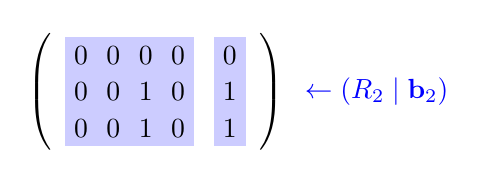
\begin{tikzpicture}[scale=0.7]
\matrix (m) [matrix of math nodes, left delimiter=(, right delimiter=), ampersand replacement=\&] {
|[fill=blue!20]| 0 \& |[fill=blue!20]| 0 \& |[fill=blue!20]| 0 \& |[fill=blue!20]| 0 \& \vrule \& |[fill=blue!20]| 0 \\
|[fill=blue!20]| 0 \& |[fill=blue!20]| 0 \& |[fill=blue!20]| 1 \& |[fill=blue!20]| 0 \& \vrule \& |[fill=blue!20]| 1 \\
|[fill=blue!20]| 0 \& |[fill=blue!20]| 0 \& |[fill=blue!20]| 1 \& |[fill=blue!20]| 0 \& \vrule \& |[fill=blue!20]| 1 \\
};
\node[right=0.5cm of m, blue] {$\leftarrow (R_2 \mid \mathbf{b}_2)$};
\end{tikzpicture}
\end{center}

\vspace{0.5em}

\x{Equation from $(R_2 \mid \mathbf{b}_2)$} (read any non-zero row):

$$x_3 = 1$$

\end{frame}

\begin{frame}[fragile]{Step 7: Final Remainder is Zero}

After subtracting $(R_2 \mid \mathbf{b}_2)$:

\begin{center}
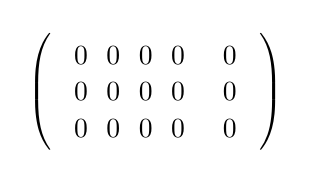
\begin{tikzpicture}[scale=0.7]
\matrix (m) [matrix of math nodes, left delimiter=(, right delimiter=), ampersand replacement=\&] {
0 \& 0 \& 0 \& 0 \& \vrule \& 0 \\
0 \& 0 \& 0 \& 0 \& \vrule \& 0 \\
0 \& 0 \& 0 \& 0 \& \vrule \& 0 \\
};
\end{tikzpicture}
\end{center}

\vspace{0.5em}

\x{Cross-filling complete}!

$$(A \mid \mathbf{b}) = (R_1 \mid \mathbf{b}_1) + (R_2 \mid \mathbf{b}_2)$$

\end{frame}

\begin{frame}{Step 8: The Matrix $V$}

Recall: $(A \mid \mathbf{b}) = UV$ where rows of $V$ come from each $(R_i \mid \mathbf{b}_i)$.

\vspace{0.5em}

\x{Explicitly}:

$$V = \begin{pmatrix}
1 & 2 & 0 & 1 & | & 5 \\
0 & 0 & 1 & 0 & | & 1
\end{pmatrix}$$

\vspace{0.5em}

\begin{itemize}
\item Row 1 from $(R_1 \mid \mathbf{b}_1)$: $x_1 + 2x_2 + 0x_3 + x_4 = 5$
\item Row 2 from $(R_2 \mid \mathbf{b}_2)$: $0x_1 + 0x_2 + x_3 + 0x_4 = 1$
\end{itemize}

\vspace{0.5em}

Solving $(A \mid \mathbf{b})$ is equivalent to solving $V$!

\end{frame}

\begin{frame}{Step 9: How to Identify Pivot and Free Variables}

From $(R_2 \mid \mathbf{b}_2)$ to $(R_1 \mid \mathbf{b}_1)$, we went from 1 active variable to 4 active variables.

\vspace{0.5em}

\x{Which new variables appeared?} $x_1, x_2, x_4$ (three new variables)

\vspace{0.5em}

\x{Which one did we choose as pivot in $(R_1 \mid \mathbf{b}_1)$?} $x_1$ (at position (1,1))

\vspace{0.5em}

Therefore:
\begin{itemize}
\item $x_1$ = \x{pivot variable} (we chose it)
\item $x_2, x_4$ = \x{free variables} (appeared but not chosen)
\end{itemize}

\vspace{1em}

\x{General rule}: From $(R_{i+1} \mid \mathbf{b}_{i+1})$ to $(R_i \mid \mathbf{b}_i)$, new variables appear. The one we chose as pivot = pivot variable. Others = free variables.

\end{frame}

\begin{frame}{Step 10: Summary of Variables}

\x{Pivot columns}: 1, 3

\begin{itemize}
\item \x{Pivot variables}: $x_1, x_3$ (determined by equations)
\end{itemize}

\vspace{1em}

\x{Non-pivot columns}: 2, 4

\begin{itemize}
\item \x{Free variables}: $x_2, x_4$ (can choose any value)
\end{itemize}

\vspace{1em}

\x{Existence check}: No equation of form $0 = c$ ($c \neq 0$) found.

$\Rightarrow$ \textbf{Solution exists!}

\end{frame}

\begin{frame}{Step 11: Backward Solving}

\x{From $(R_2 \mid \mathbf{b}_2)$ (simplest equation)}:

$$x_3 = 1$$

\vspace{1em}

\x{From $(R_1 \mid \mathbf{b}_1)$}:

$$x_1 + 2x_2 + 0x_3 + x_4 = 5$$

Substituting $x_3 = 1$:

$$x_1 + 2x_2 + 0(1) + x_4 = 5$$

$$x_1 + 2x_2 + x_4 = 5$$

Solve for pivot variable $x_1$:

$$x_1 = 5 - 2x_2 - x_4$$

\end{frame}

\begin{frame}{Step 12: Write General Solution}

Let free variables $x_2 = s$ and $x_4 = t$ (parameters).

\vspace{0.5em}

\x{General solution}:

$$\mathbf{x} = \begin{pmatrix} x_1 \\ x_2 \\ x_3 \\ x_4 \end{pmatrix} = \begin{pmatrix} 5 - 2s - t \\ s \\ 1 \\ t \end{pmatrix}$$

\vspace{1em}

Decompose:

$$= \begin{pmatrix} 5 \\ 0 \\ 1 \\ 0 \end{pmatrix} + s\begin{pmatrix} -2 \\ 1 \\ 0 \\ 0 \end{pmatrix} + t\begin{pmatrix} -1 \\ 0 \\ 0 \\ 1 \end{pmatrix}$$

\end{frame}

\begin{frame}{Step 13: Interpret the Solution}

$$\mathbf{x} = \underbrace{\begin{pmatrix} 5 \\ 0 \\ 1 \\ 0 \end{pmatrix}}_{\text{Particular solution } \mathbf{x}_p} + s\underbrace{\begin{pmatrix} -2 \\ 1 \\ 0 \\ 0 \end{pmatrix}}_{\text{Null vector } \mathbf{v}_1} + t\underbrace{\begin{pmatrix} -1 \\ 0 \\ 0 \\ 1 \end{pmatrix}}_{\text{Null vector } \mathbf{v}_2}$$

\vspace{1em}

\x{Particular solution} ($s = t = 0$): $\mathbf{x}_p = \begin{pmatrix} 5 \\ 0 \\ 1 \\ 0 \end{pmatrix}$

\vspace{0.5em}

\x{Null space basis}:
$$\text{Null}(A) = \text{span}\left\{\begin{pmatrix} -2 \\ 1 \\ 0 \\ 0 \end{pmatrix}, \begin{pmatrix} -1 \\ 0 \\ 0 \\ 1 \end{pmatrix}\right\}$$

\vspace{0.5em}

\x{Uniqueness}: Two free variables $\to$ \textbf{infinitely many solutions}.

\end{frame}

% ═══════════════════════════════════════
% §4 APPLICATIONS
% ═══════════════════════════════════════
\section{Applications: Existence, Uniqueness, Null Space}

\begin{frame}{Application 1: Finding Null Space Basis}

\begin{prop}
To find a basis for $\text{Null}(A)$:

\begin{enumerate}
\item Solve $A\mathbf{x} = \mathbf{0}$ using cross-filling
\item Identify free variables
\item For each free variable, set it = 1, others = 0
\item Solve for pivot variables
\end{enumerate}

Result: $\text{Null}(A) = \text{span}\{\mathbf{v}_1, \ldots, \mathbf{v}_k\}$

\x{Descriptive $\to$ Constructive conversion complete!}
\end{prop}

\end{frame}

\begin{frame}{Application 1: Concrete Example}

From our example, free variables are $x_2, x_4$.

\vspace{1em}

\x{For $\mathbf{v}_1$}: Set $x_2 = 1, x_4 = 0$

\begin{align*}
x_3 &= 1 \quad \text{wait, this is for } A\mathbf{x} = \mathbf{b}\text{!}
\end{align*}

\x{Correction}: For null space, solve $A\mathbf{x} = \mathbf{0}$ (not $\mathbf{b}$)!

\vspace{0.5em}

From $(R_1 \mid \mathbf{0})$: $x_1 + 2x_2 + x_4 = 0$, so $x_1 = -2x_2 - x_4$

From $(R_2 \mid \mathbf{0})$: $x_3 = 0$

Set $x_2 = 1, x_4 = 0$: $\mathbf{v}_1 = \begin{pmatrix} -2 \\ 1 \\ 0 \\ 0 \end{pmatrix}$

Set $x_2 = 0, x_4 = 1$: $\mathbf{v}_2 = \begin{pmatrix} -1 \\ 0 \\ 0 \\ 1 \end{pmatrix}$

\end{frame}

\begin{frame}{Application 2: Existence Criterion — The Key Insight}

\x{Question}: When does $A\mathbf{x} = \mathbf{b}$ have a solution?

\vspace{1em}

\x{Strategy}: Cross-fill $(A \mid \mathbf{b})$ using pivots from $A$ only.

\vspace{0.5em}

\begin{itemize}
\item Use $r = \text{rank}(A)$ pivots to eliminate $A$ part
\item After $r$ steps, all pivot rows are cleared
\item Then check: \x{What's left in the non-pivot rows?}
\end{itemize}

\vspace{1em}

Let's see this visually with colored rows$\ldots$

\end{frame}

\begin{frame}[fragile]{Case 1: All Equations Effective (Solution Exists)}

After using $r$ pivots from $A$:

\begin{center}
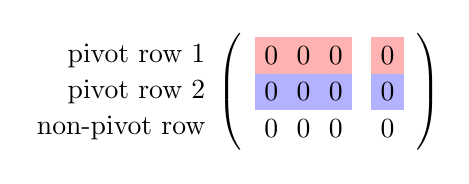
\begin{tikzpicture}[scale=0.7]
% Pivot rows (colored)
\matrix (m) [matrix of math nodes, left delimiter=(, right delimiter=), ampersand replacement=\&] {
|[fill=red!30]| 0 \& |[fill=red!30]| 0 \& |[fill=red!30]| 0 \& \vrule \& |[fill=red!30]| 0 \\
|[fill=blue!30]| 0 \& |[fill=blue!30]| 0 \& |[fill=blue!30]| 0 \& \vrule \& |[fill=blue!30]| 0 \\
0 \& 0 \& 0 \& \vrule \& 0 \\
};
\node[left=0.5cm of m-1-1] {pivot row 1};
\node[left=0.5cm of m-2-1] {pivot row 2};
\node[left=0.5cm of m-3-1] {non-pivot row};
\end{tikzpicture}
\end{center}

\vspace{0.5em}

\x{Observation}:
\begin{itemize}
\item Pivot rows (colored): cleared by design
\item Non-pivot rows: \x{passively became 0} (including $\mathbf{b}$ part)
\end{itemize}

\x{Conclusion}: No equation of form $0 = c$ ($c \neq 0$).

All equations are \textbf{effective} (not contradictory).

\x{Solution exists!}

\end{frame}

\begin{frame}[fragile]{Case 2: Contradiction Appears (No Solution)}

After using $r$ pivots from $A$:

\begin{center}
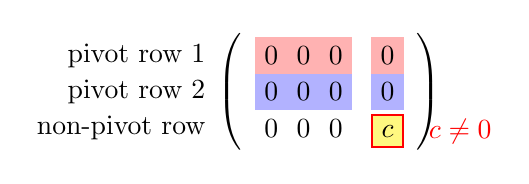
\begin{tikzpicture}[scale=0.7]
% Pivot rows (colored) + non-pivot with contradiction
\matrix (m) [matrix of math nodes, left delimiter=(, right delimiter=), ampersand replacement=\&] {
|[fill=red!30]| 0 \& |[fill=red!30]| 0 \& |[fill=red!30]| 0 \& \vrule \& |[fill=red!30]| 0 \\
|[fill=blue!30]| 0 \& |[fill=blue!30]| 0 \& |[fill=blue!30]| 0 \& \vrule \& |[fill=blue!30]| 0 \\
0 \& 0 \& 0 \& \vrule \& |[fill=yellow!50]| c \\
};
\node[left=0.5cm of m-1-1] {pivot row 1};
\node[left=0.5cm of m-2-1] {pivot row 2};
\node[left=0.5cm of m-3-1] {non-pivot row};
\draw[thick, red] (m-3-5.south west) rectangle (m-3-5.north east);
\node[right=0.2cm of m-3-5, red] {$c \neq 0$};
\end{tikzpicture}
\end{center}

\vspace{0.5em}

\x{Observation}:
\begin{itemize}
\item Pivot rows: cleared
\item Non-pivot row: $A$ part is 0, but $\mathbf{b}$ part $\neq$ 0
\end{itemize}

This gives equation: $0 = c$ where $c \neq 0$ — \x{contradiction!}

\x{No solution!}

\end{frame}

\begin{frame}{Existence Theorem: Correct Logic}

\begin{thm}[Existence of Solutions]
$A\mathbf{x} = \mathbf{b}$ has a solution if and only if:

$$\text{rank}(A \mid \mathbf{b}) = \text{rank}(A)$$
\end{thm}

\vspace{1em}

\x{Correct logic}:

\begin{itemize}
\item The cross-filling algorithm \textbf{always proceeds}
\item If rank$(A \mid \mathbf{b})$ = rank$(A)$ $\Rightarrow$ no contradiction $\Rightarrow$ solution exists
\item If rank$(A \mid \mathbf{b})$ = rank$(A) + 1$ $\Rightarrow$ contradiction $0 = c$ appears $\Rightarrow$ \textbf{any $\mathbf{x}$ violates this equation} $\Rightarrow$ no solution
\end{itemize}

\end{frame}

\begin{frame}{Geometric Interpretation}

$$\mathbf{b} \in \text{Col}(A) \iff \text{rank}(A \mid \mathbf{b}) = \text{rank}(A)$$

\vspace{1em}

Adding $\mathbf{b}$ as a column doesn't increase rank $\iff$ $\mathbf{b}$ is already in span of $A$'s columns.

\vspace{1em}

\x{Coffee shop}: Customer's ingredient list is achievable $\iff$ it's in our column space.

\end{frame}

\begin{frame}{Application 3: Uniqueness Criterion}

\begin{thm}[Uniqueness of Solutions]
If $A\mathbf{x} = \mathbf{b}$ has a solution, it is \textbf{unique} if and only if:

$$\text{Null}(A) = \{\mathbf{0}\}$$

Equivalently:
\begin{itemize}
\item No free variables
\item All columns are pivot columns
\item $\text{rank}(A) = n$ (number of columns)
\end{itemize}
\end{thm}

\vspace{0.5em}

\x{Proof idea}: If $\mathbf{x}_1, \mathbf{x}_2$ are both solutions, then $\mathbf{x}_1 - \mathbf{x}_2 \in \text{Null}(A)$.

\end{frame}

\begin{frame}{Application 4: Structure of Solution Set}

\begin{thm}[General Solution Structure]
If $A\mathbf{x} = \mathbf{b}$ has solutions, \textbf{all solutions} have the form:

$$\mathbf{x} = \mathbf{x}_p + \mathbf{x}_n$$

where:
\begin{itemize}
\item $\mathbf{x}_p$ is any \textbf{particular solution}
\item $\mathbf{x}_n \in \text{Null}(A)$ is arbitrary
\end{itemize}
\end{thm}

\vspace{0.5em}

\x{Geometric picture}: Solution set is $\mathbf{x}_p + \text{Null}(A)$ (affine subspace).

\end{frame}

% ═══════════════════════════════════════
% §5 RANK-NULLITY
% ═══════════════════════════════════════
\section{Dimension Formula: Rank-Nullity Theorem}

\begin{frame}{Counting Pivot and Free Variables}

From cross-filling an $m \times n$ matrix $A$:

\begin{itemize}
\item Number of pivot columns = $\text{rank}(A)$
\item Number of free variables = $\dim(\text{Null}(A))$
\item Total columns = $n$
\end{itemize}

\vspace{1em}

Every column is either pivot or non-pivot:

$$\text{rank}(A) + \dim(\text{Null}(A)) = n$$

\vspace{1em}

This is the \x{Rank-Nullity Theorem}.

\end{frame}

\begin{frame}[fragile]{Visual Example: Rank-Nullity}

From our example:

\begin{center}
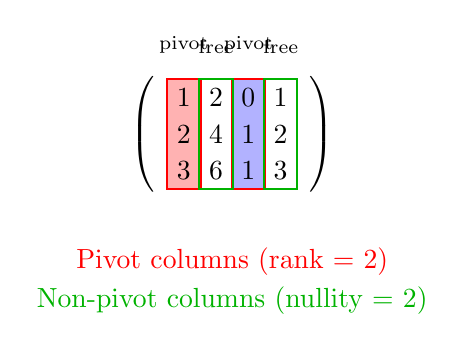
\begin{tikzpicture}[scale=0.8]
\matrix (m) [matrix of math nodes, left delimiter=(, right delimiter=), ampersand replacement=\&] {
|[fill=red!30]| 1 \& 2 \& |[fill=blue!30]| 0 \& 1 \\
|[fill=red!30]| 2 \& 4 \& |[fill=blue!30]| 1 \& 2 \\
|[fill=red!30]| 3 \& 6 \& |[fill=blue!30]| 1 \& 3 \\
};
\node[above=0.2cm of m-1-1] {\scriptsize pivot};
\node[above=0.2cm of m-1-2] {\scriptsize free};
\node[above=0.2cm of m-1-3] {\scriptsize pivot};
\node[above=0.2cm of m-1-4] {\scriptsize free};

\draw[red, thick] (m-1-1.north west) rectangle (m-3-1.south east);
\draw[red, thick] (m-1-3.north west) rectangle (m-3-3.south east);
\node[below=0.5cm of m, red] {Pivot columns (rank = 2)};

\draw[green!70!black, thick] (m-1-2.north west) rectangle (m-3-2.south east);
\draw[green!70!black, thick] (m-1-4.north west) rectangle (m-3-4.south east);
\node[below=1cm of m, green!70!black] {Non-pivot columns (nullity = 2)};
\end{tikzpicture}
\end{center}

\vspace{0.5em}

$$\underbrace{2}_{\text{rank}} + \underbrace{2}_{\text{nullity}} = \underbrace{4}_{n}$$

\end{frame}

\begin{frame}{Rank-Nullity Theorem}

\begin{thm}[Rank-Nullity Theorem]
For any $m \times n$ matrix $A$:

$$\boxed{\text{rank}(A) + \dim(\text{Null}(A)) = n}$$
\end{thm}

\vspace{1em}

\x{Proof idea}: Every column is either:
\begin{itemize}
\item A pivot column (contributes to rank), or
\item A non-pivot column (contributes one basis vector to null space)
\end{itemize}

These counts sum to $n$.

\end{frame}

% ═══════════════════════════════════════
% §6 ORTHOGONALITY
% ═══════════════════════════════════════
\section{Preview: Null Space and Row Space Orthogonality}

\begin{frame}{Natural Orthogonality}

\begin{thm}
$\text{Null}(A) \perp \text{Row}(A)$

Every vector in $\text{Null}(A)$ is orthogonal to every vector in $\text{Row}(A)$.
\end{thm}

\vspace{1em}

\x{Proof}: Let $\mathbf{x} \in \text{Null}(A)$ and $\mathbf{r}_i$ = $i$-th row.

By definition: $A\mathbf{x} = \mathbf{0}$ means $\mathbf{r}_i \cdot \mathbf{x} = 0$ for all $i$.

\end{frame}

\begin{frame}{Coffee Shop Interpretation}

If $A$ = "drinks $\to$ ingredients":

\begin{itemize}
\item \textbf{Row space}: All ingredient combinations from drinks
\item \textbf{Null space}: Relationships between drinks (which can be made from others)
\end{itemize}

\vspace{1em}

\x{Perpendicular}: A relationship (which drinks are equivalent) has nothing in common with actual ingredient requirements!

\vspace{1em}

\x{Next lecture}: Four fundamental subspaces and complete orthogonal structure.

\end{frame}

% ═══════════════════════════════════════
% §7 SUMMARY
% ═══════════════════════════════════════
\section{Summary}

\begin{frame}{What We Achieved Today}

\x{1. Null Space}:
\begin{itemize}
\item Descriptive: $\{\mathbf{x} : A\mathbf{x} = \mathbf{0}\}$
\item Records relationships between columns
\item Conversion to constructive requires solving
\end{itemize}

\vspace{0.5em}

\x{2. Cross-Filling Method}:
\begin{itemize}
\item Each $(R_i \mid \mathbf{b}_i)$ = one equation
\item Matrix $V$ explicitly shows simplified equations
\item Variables decrease (at least one per step) $\to$ backward solving
\end{itemize}

\end{frame}

\begin{frame}{What We Achieved Today (continued)}

\x{3. Existence}: rank$(A \mid \mathbf{b})$ = rank$(A)$ $\iff$ no contradiction

\begin{itemize}
\item Visual: pivot rows cleared, non-pivot rows passive
\item If non-pivot row has $0 = c$ ($c \neq 0$) $\to$ no solution
\end{itemize}

\vspace{0.5em}

\x{4. Uniqueness}: $\text{Null}(A) = \{\mathbf{0}\}$ $\iff$ unique solution

\vspace{0.5em}

\x{5. Rank-Nullity}: rank$(A)$ + nullity = $n$ (visual: colored columns)

\vspace{0.5em}

\x{6. Orthogonality}: $\text{Null}(A) \perp \text{Row}(A)$

\vspace{1em}

\x{Next lecture}: Four fundamental subspaces!

\end{frame}

\end{document}
